\chapter{Autonomous Driving}\label{Ch:ResultsCarRacing}

After verifying the correctness of our implementation by applying it to simpler environments such as Cart Pole and Breakout, we moved on to working on OpenAI's CarRacing environment, which is a 2-dimensional car racing game. In section \ref{sec1}, we go over the CarRacing environment in detail. We explore the effect of neural network structure, action space and reward feedback in the following sections.

\section{The OpenAI CarRacing Environment}\label{sec1}
\begin{figure}[h!]
\centering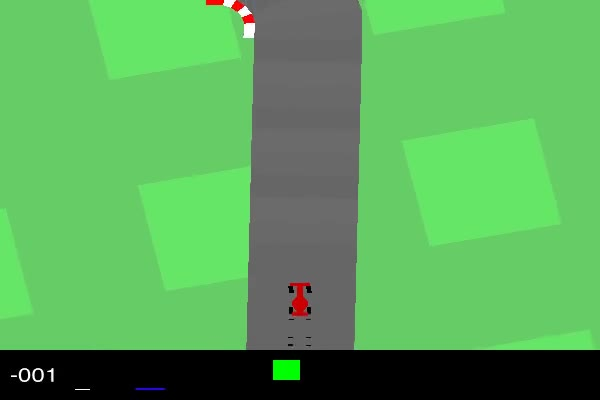
\includegraphics[scale=0.45,clip]{Graphics/carracing.jpg}
\caption[Car Racing]{The game environment of the car racing game}
\label{fig:carracing}
\end{figure}
In OpenAI's CarRacing environment - from here on referred to as the `car racing game' - the emulator provides 96 by 96 RGB screenshots to the agent, which has control over a red racing car, as shown in Figure \ref{fig:carracing}. Notice that the track is made up of distinct tiles. The reward signal is -0.1 for every frame passed and $\frac{1000}{N}$ for every tile visited, where N is the total number of tiles on the track. Thus the goal of the game is to finish the track as fast as possible, without missing any of the tiles. The actions come in the form of an array of three numbers. In the array, the first number indicates steer, the second number indicates acceleration and the third number indicates deceleration. The steer coordinate is continuous from -1 to 1 while the acceleration and the deceleration are continuous from 0 to 1. For example, if the agent finishes in 732 frames and never leaves the track doing so, the reward is 1000 - 0.1*732 = 926.8 points. The episode finishes when all tiles are visited or more than 1000 frames pass. As per OpenAI's guidelines, the environment is solved when an average score of 900 or more is achieved over 100 episodes. 
\par
We chose this environment for several reasons: first, the car racing game is similar to real life autonomous driving; second, the game environment can be easily altered, allowing for interesting exploration of robustness of Deep RL methods; third, according to the leaderboard on OpenAI's website, no one has successfully solved the game. 
\par
To be able to iterate faster, we created four different types of training environment of varying complexity: random short tracks, fixed one track, fixed three tracks and random tracks. In the random short track environment, there are 50 tiles for the agent to finish while in the other environments, there are approximately 300 tiles. Random short tracks and random tracks environment display randomly generated tracks for each episode while the other environments display the same one (fixed one track) or three tracks (fixed three tracks).

\section{Network Architecture}
When we first started working on the car racing environment, the 2 convolutional layer architecture used in Chapter 4 and \cite{mnih2013playing} was used. However, considering the complexity of the game, a deeper three-convolutional architecture was tested.

\begin{figure}[h]
\centering
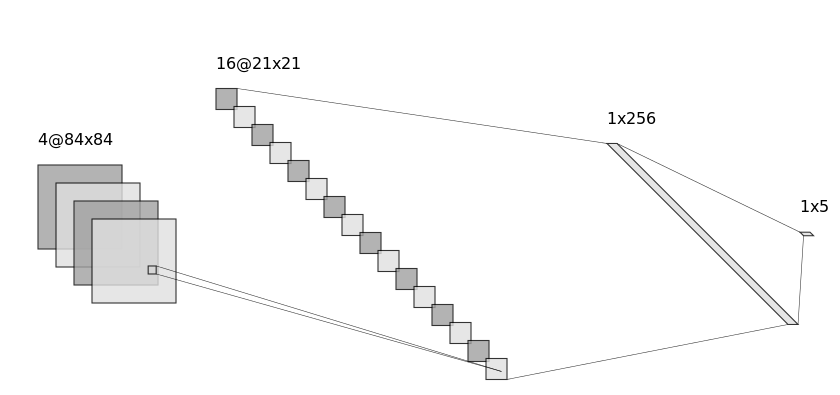
\includegraphics[width=0.6\textwidth]{Graphics/nn_crop2.png}
\caption[Two Convolutional Neural Network Structure]{Neural Network with two convolutional layers. Specific parameters are in Table \ref{table: neuralstructures}.}
\label{fig:2conv}
\end{figure}

\begin{figure}[h]
\centering
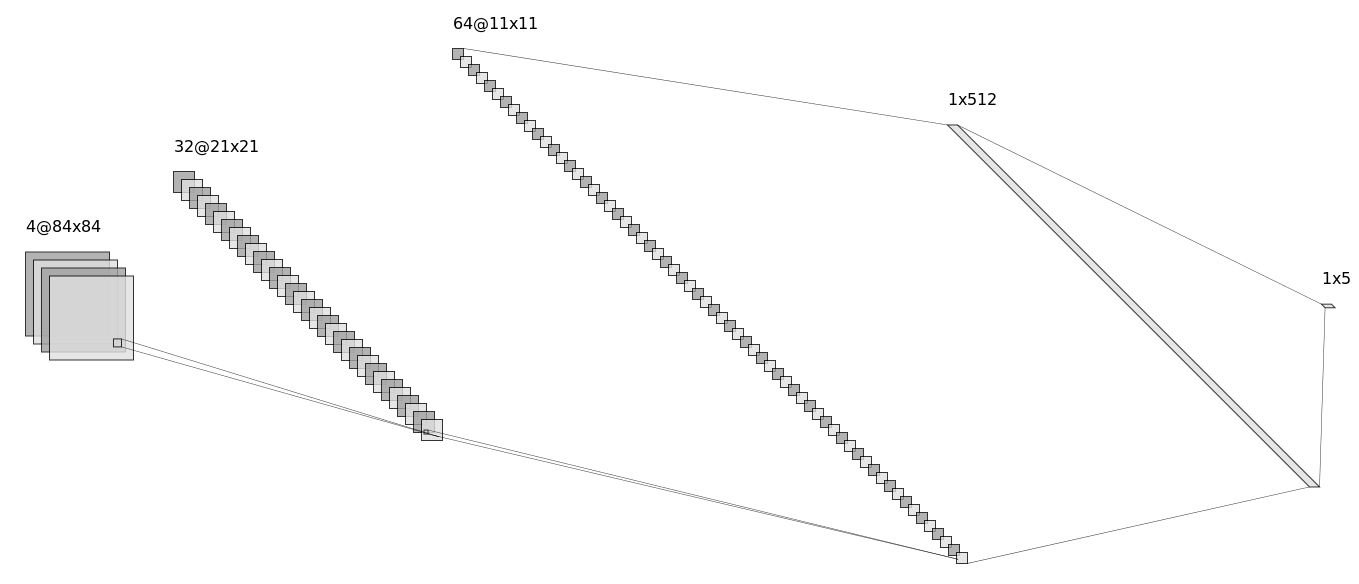
\includegraphics[width=0.6\textwidth]{Graphics/nn_crop3.png}
\caption[Three Convolutional Neural Network Structure]{Neural Network with three convolutional layers. Specific parameters are in Table \ref{table: neuralstructures}.}
\label{fig:3conv}
\end{figure}

We trained these two neural network structures in the random short tracks environment. 

\begin{figure}[h]
\centering
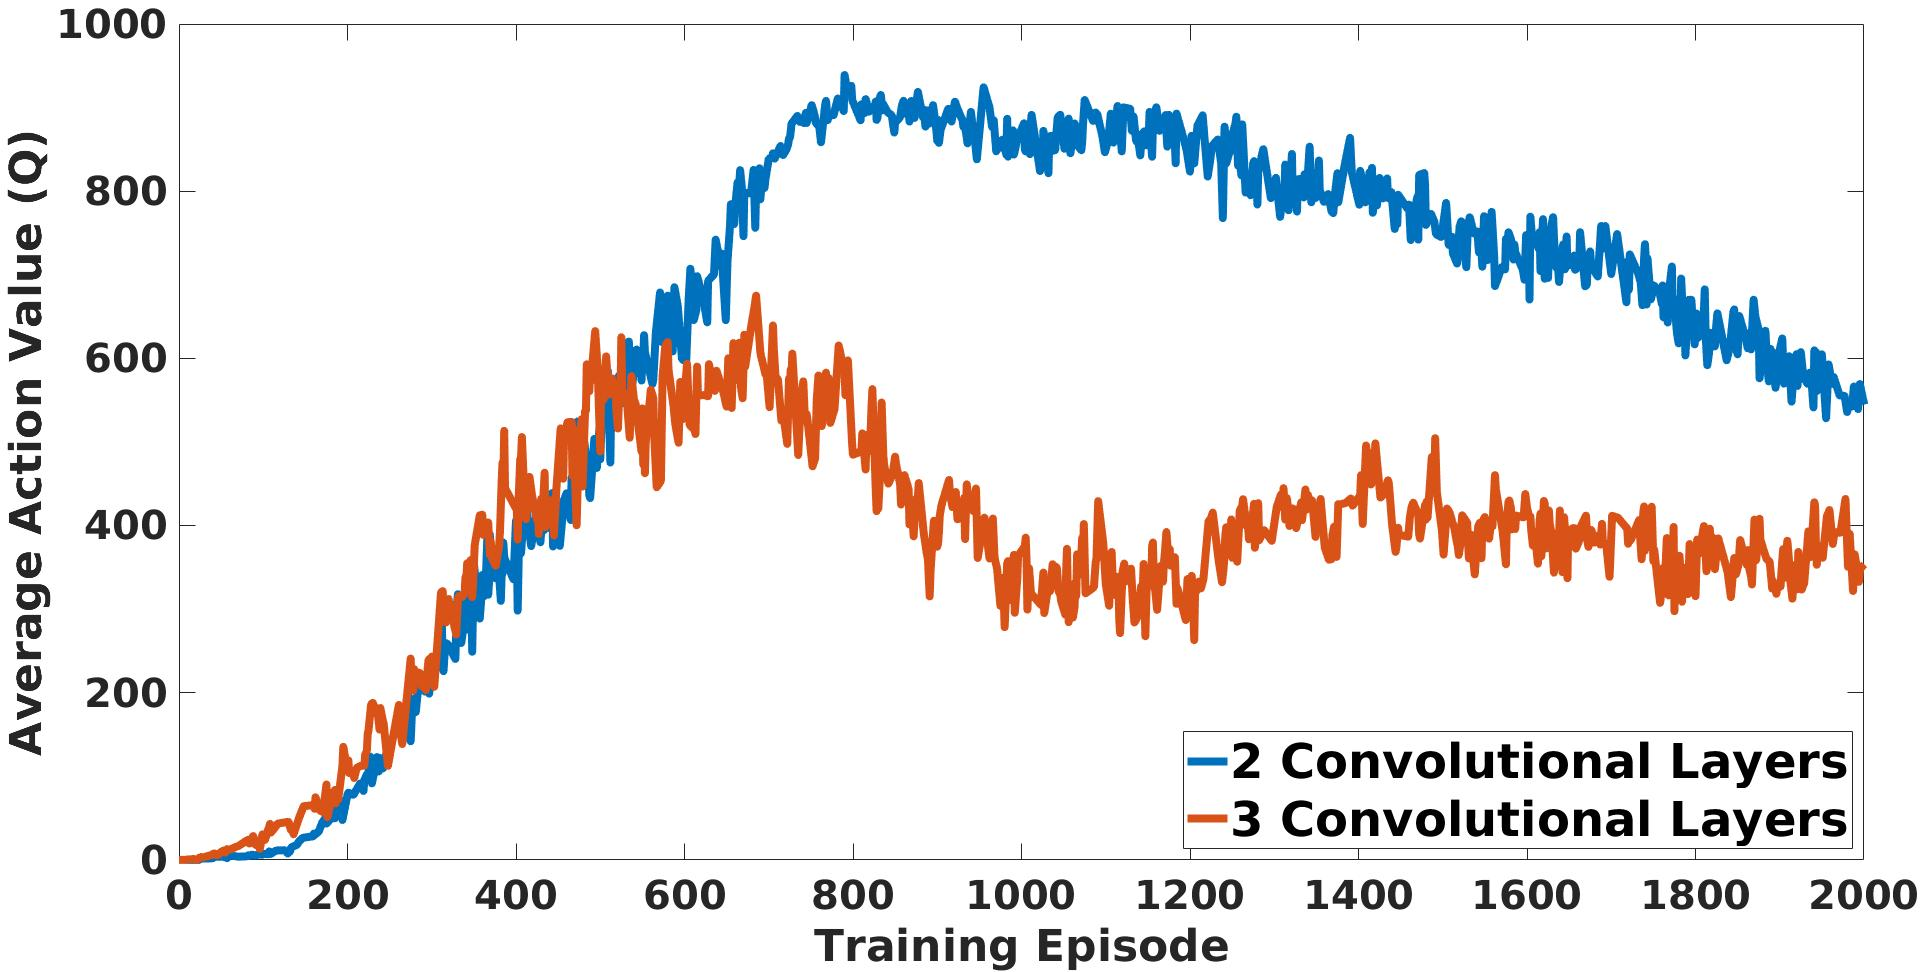
\includegraphics[width=0.6\textwidth]{Graphics/AveQ_conv.jpg}
\caption[Average Action Values Neural Network Structure Comparison]{Average action values using two convolutional layers (orange) and three layers (blue).}
\label{fig:conv_aveq}
\end{figure}

\begin{figure}[h]
\centering
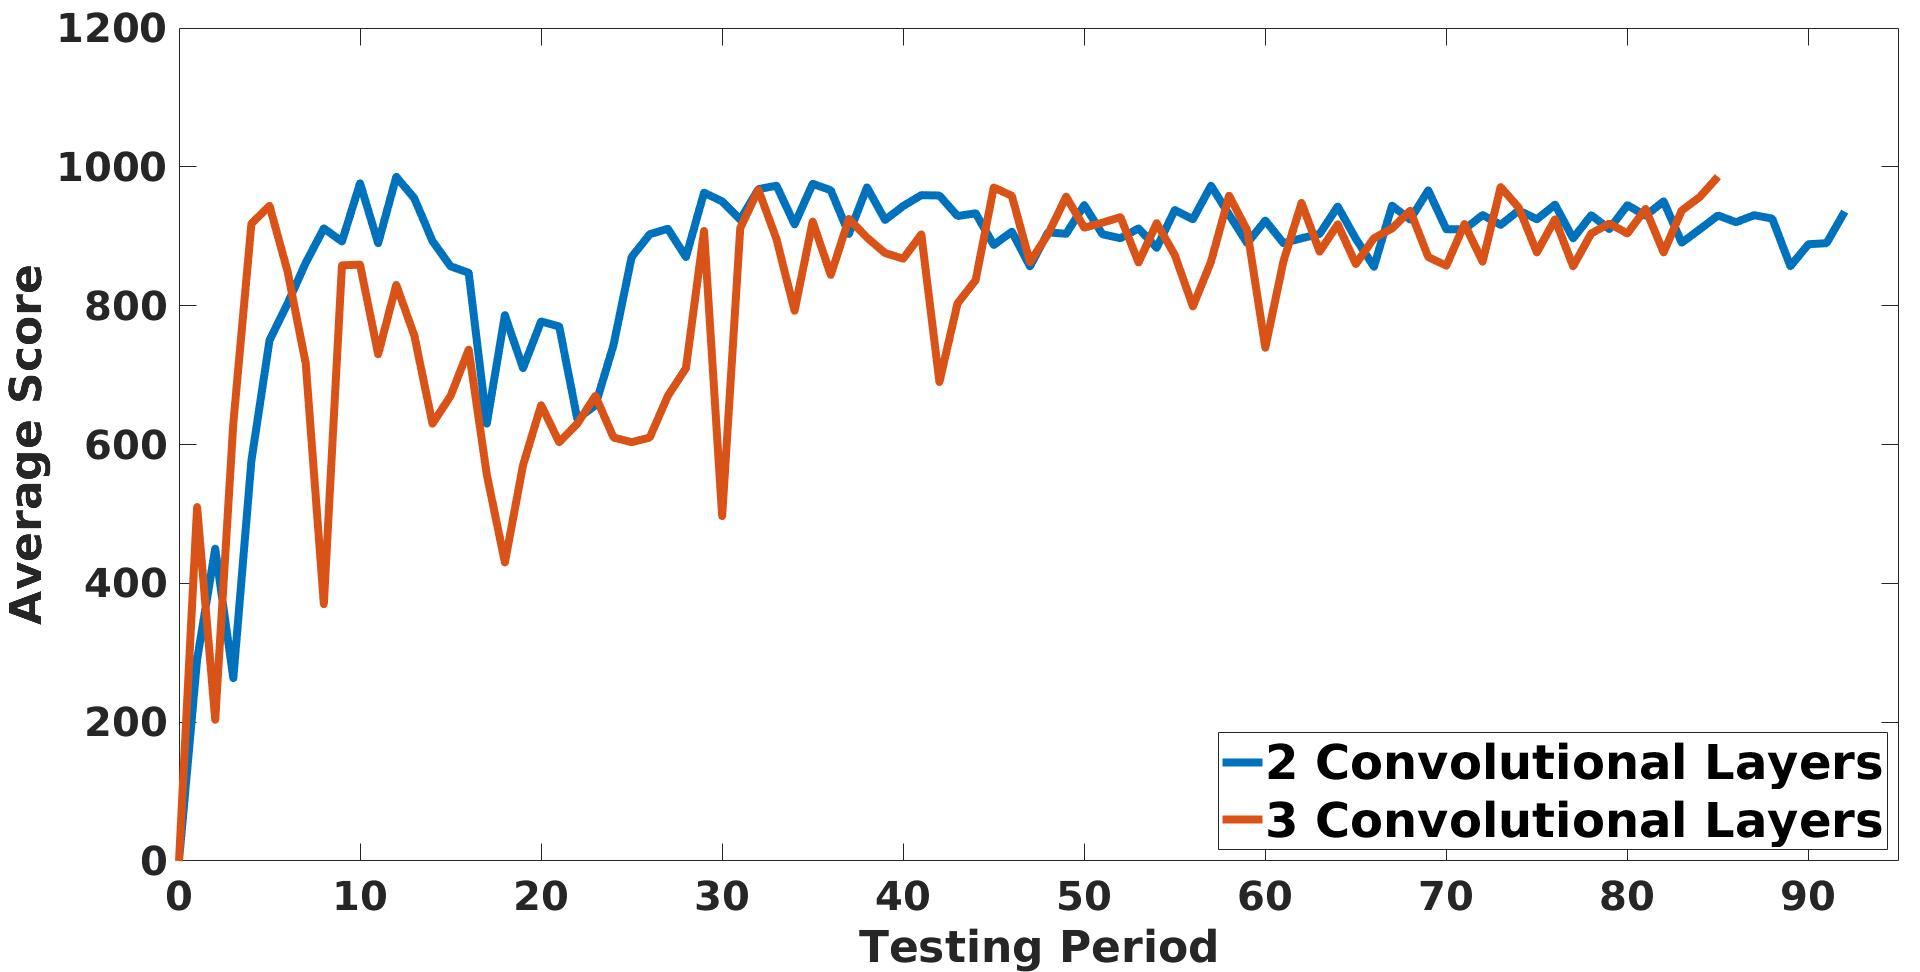
\includegraphics[width=0.6\textwidth]{Graphics/TestScore_conv.jpg}
\caption[Average Test Score Neural Network Structure Comparison]{Average score over five tests using two convolutional layers (orange) and three layers (blue).}
\label{fig:conv_test}
\end{figure}

As shown in Figure \ref{fig:conv_test}, the model with two convolutional layers didn't perform as well as the one with three convolutional layers. The model with two convolutional layers also took longer to converge, judging on the trend of average Q-values. Therefore, we believe that three convolutional layers are better at identifying important features in the input, thus we decided to continue our investigation using the deeper architecture.

\section{Action Space}
The action space in the car racing game is continuous. But when human plays the game, the only available actions are right turn, left turn, acceleration and deceleration. We started experiments with these four actions. However, we soon realized that human players can also choose not to input any actions (no operation). In order to compare the effect of having four with five actions, we conduct a test once again on the random short track environment.

\begin{figure}[h]
\centering
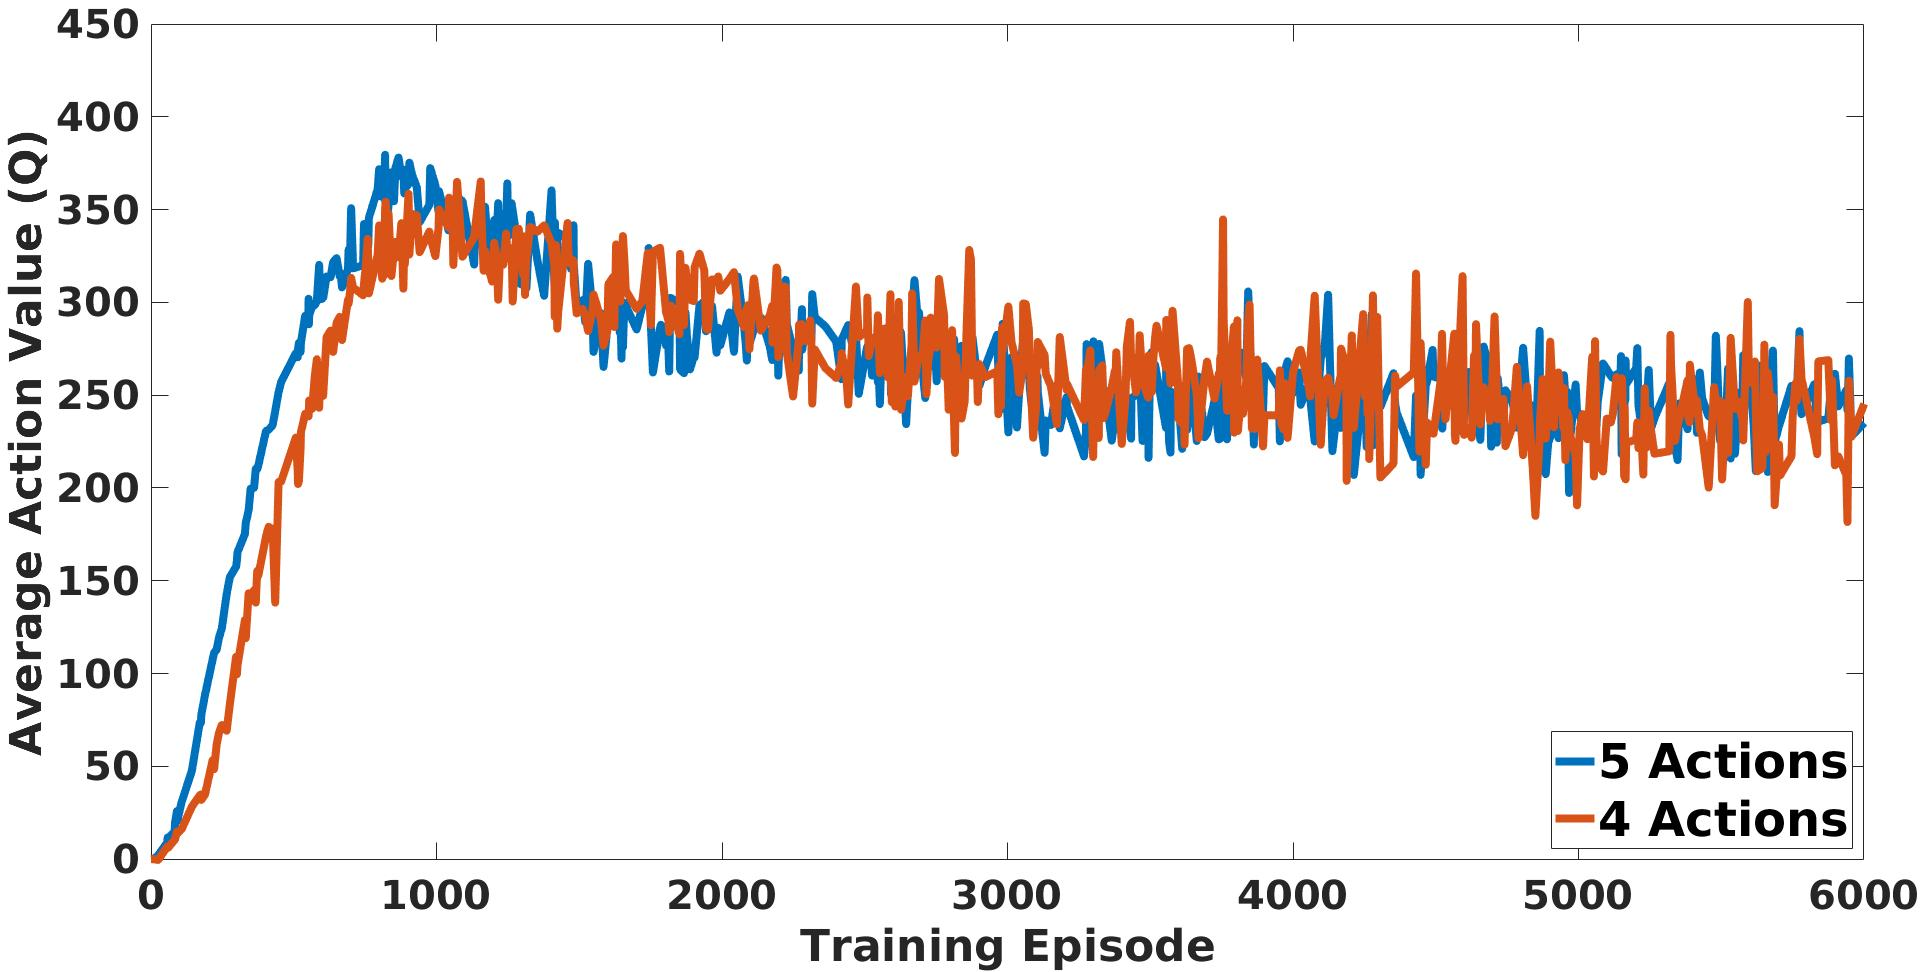
\includegraphics[width=0.6\textwidth]{Graphics/AveQ_action.jpg}
\caption[Average Action Values Action Space Comparison]{Average action values using four (orange) and five (blue) actions.
Specific parameters are included in Table \ref{table: ActionSpace}}
\label{fig:action_test}
\end{figure}

\begin{figure}[h]
\centering
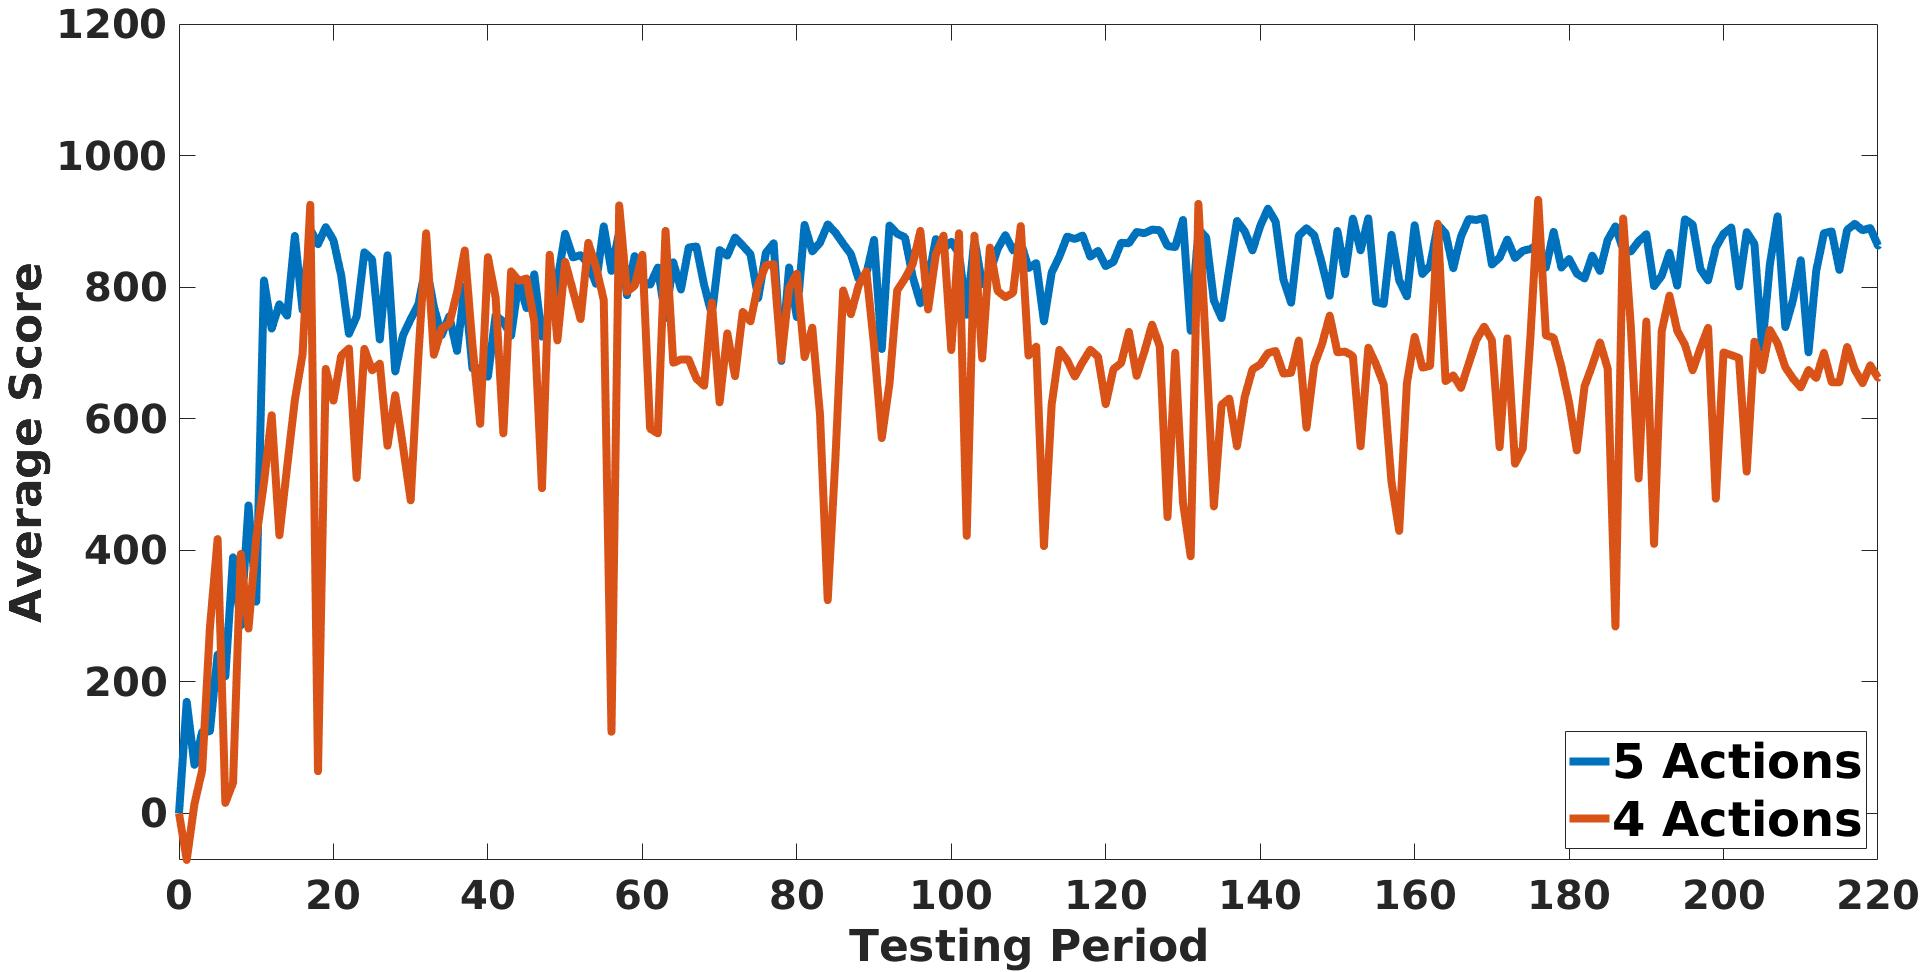
\includegraphics[width=0.6\textwidth]{Graphics/TestScore_action.jpg}
\caption[Average Test Score Action Space Comparison]{Average scores over five tests using four (orange) and five (blue) actions.
Specific parameters are included in Table \ref{table: ActionSpace}}
\label{fig:action_aveq}
\end{figure}

As shown in Figure \ref{fig:action_aveq}, the model with five actions achieves better average scores over five tests after 120 testing periods. Hence we resolved to use five actions for models.

\newpage
\section{Reward}
The nature of the reward signal from the environment greatly influences the convergence and performance of RL models. Therefore, we progressed to investigate the effect that rewards have on the performance in the car racing game. As mentioned in section \ref{sec1}, in the original game there are two different kinds of rewards the agent can receive. For every tile the car visits, the reward is 1000/N, where N is the total number of tiles on the track, while for every frame passed, the reward is -0.1. 
\par
Intuitively, if the reward for visiting tiles is magnified, the agent will tend to visit all tiles at the cost of possibly slowing down. If the negative reward for one frame passed is magnified, the agent will be encouraged to go faster while possibly missing some of the tiles. Therefore, we experimented with changing the ratio and magnitudes of positive and negative rewards. 
\par 
We trained models with six different pairs of positive and negative rewards. We then tested the trained models on 100 random tracks and compared the average scores and standard deviations. As shown in Figure \ref{fig:rewardclip}, when the positive reward for visiting one tile is fixed to 1, the performance worsens as the magnitude of the negative reward decreases. When the negative reward is fixed to -0.1, the performance varies when the positive reward changes from 20 to 1. We suspect there is a better reward pair, with positive reward between 1 and 10 and negative reward being 0.1. 
\newpage
\begin{figure}[h!]
\centering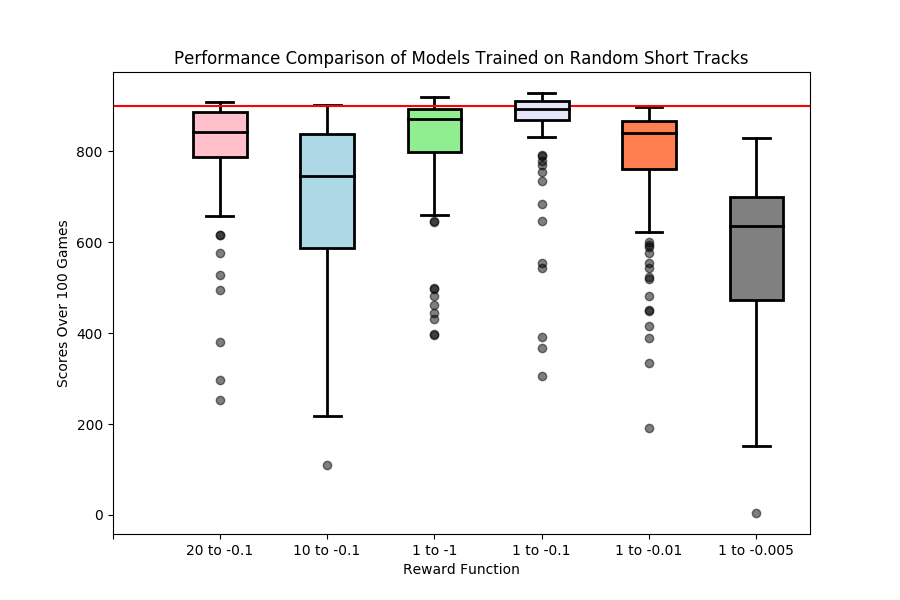
\includegraphics[scale=0.5,clip]{Graphics/performance_clip_reward.png}
\caption[Clip Reward Performance]{Performance of models with different reward ratios trained in the random short track environment.}\label{fig:rewardclip}
\end{figure}

\endinput


